\thispagestyle{cackithitoannone}
\pagestyle{cackithitoan}
\everymath{\color{cackithi}}
\graphicspath{{../cackithi/pic/}}
\begingroup
\AddToShipoutPicture*{\put(0,616){
\includegraphics[width=19.3cm]{../bannercackithi}}} 
\AddToShipoutPicture*{\put(150,575){
\includegraphics[scale=1]{../tieude1.pdf}}}
\centering
\endgroup
\vspace*{130pt}

\begin{multicols}{2}
	Trong phần đầu chuyên mục, chúng tôi sẽ trình bày lời giải của các bài toán trong kỳ thi Olympic Toán học Trẻ của Estonia năm học $2020-2021$, đăng trong số báo $10/2022$. 
	\vskip 0.1cm
	{\bf\color{cackithi} OC$\pmb{22.}$} Tia phân giác tại đỉnh $A$ của tam giác $ABC$ cắt đường tròn ngoại tiếp tam giác $ABC$ tại điểm $F (F \neq A).$ Lấy điểm $D$ và $E$ lần lượt trên các cạnh $AB$ và $AC$ sao cho $DE$ song song với $BC$. Gọi $G$ và $H$ lần lượt là giao điểm của các tia $FD$ và $FE$ với đường tròn ngoại tiếp tam giác $ABC (G \neq F, H \neq F).$ Các đường tròn ngoại tiếp tam giác $AGD$ và $AHE$ cắt nhau tại điểm $P (P \neq A).$ Chứng minh rằng điểm $P$ nằm trên đường thẳng $AF.$
	\begin{figure}[H]
		\vspace*{-10pt}
		\centering
		\captionsetup{labelformat= empty, justification=centering}
		\begin{tikzpicture}[cackithi,scale=0.95, node font=/small]
			\draw [shift={(3.46,2.88)}] (0,0) -- (-80.54882573391929:0.4) arc (-80.54882573391929:-44.21517539700811:0.4) -- cycle;
			\draw [shift={(3.46,2.88)}] (0,0) -- (-116.88247607083048:0.5) arc (-116.88247607083048:-80.54882573391929:0.5) -- cycle;
			\draw  (3.46,2.88)-- (2.,0.);
			\draw  (2.,0.)-- (6.42,0.);
			\draw  (3.46,2.88)-- (6.42,0.);
			\draw  (4.21,0.6897222222222221) circle (2.315127802914379cm);
			\draw  (3.46,2.88)-- (4.21,-1.6254055806921568);
			\draw  (2.485169230769231,0.9570461538461539)-- (5.436547750464446,0.9568724590075657);
			\draw  (2.0714369973952342,1.576494474673352)-- (4.21,-1.6254055806921568);
			\draw  (4.21,-1.6254055806921568)-- (6.0044579560443,2.1525063443046544);
			\draw  (2.0714369973952342,1.576494474673352)-- (3.46,2.88);
			\draw  (3.46,2.88)-- (6.0044579560443,2.1525063443046544);
			\draw  (2.0714369973952342,1.576494474673352)-- (6.42,0.);
			\draw  (2.,0.)-- (6.0044579560443,2.1525063443046544);
			\draw [fill=white] (3.46,2.88) circle (1.5pt);
			\draw (3.48,3.35) node {$A$};
			\draw [fill=white] (2.,0.) circle (1.5pt);
			\draw (1.66,-0.11) node {$B$};
			\draw [fill=white] (6.42,0.) circle (1.5pt);
			\draw (6.7,-0.07) node {$C$};
			\draw [fill=white] (4.21,-1.6254055806921568) circle (1.5pt);
			\draw (4.24,-1.85) node {$F$};
			\draw [fill=white] (2.485169230769231,0.9570461538461539) circle (1.5pt);
			\draw (2.48,0.65) node {$D$};
			\draw [fill=white] (5.436547750464446,0.9568724590075657) circle (1.5pt);
			\draw (5.44,0.63) node {$E$};
			\draw [fill=white] (2.0714369973952342,1.576494474673352) circle (1.5pt);
			\draw (1.64,1.73) node {$G$};
			\draw [fill=white] (6.0044579560443,2.1525063443046544) circle (1.5pt);
			\draw (6.28,2.39) node {$H$};
			\draw [fill=white] (3.7800041573402137,0.9569699500850757) circle (1.5pt);
			\draw (3.6,0.73) node {$L$};
			\draw [fill=white] (3.939424096524548,0.) circle (1.5pt);
			\draw (4.16,-0.17) node {$K$};
		\end{tikzpicture}
		\vspace*{-10pt}
	\end{figure}
	\textit{Lời giải.} 
	Ta gọi $K, L$ lần lượt là giao điểm của $AF$ với $BC, DE.$
	Theo giả thiết $AF$ là phân giác của góc $\angle BAC$ nên ta có:
	\begin{align*}
		\angle AHF&=\angle ACB \!+\! \angle BCF\\
		&= \angle ACK \!+\! \angle KAC \!=\! 180^\circ \!-\!\angle AKC.
	\end{align*}   
	Mặt khác do $DE$ song song với $BC$ nên $\angle ALE = \angle AKC.$ Từ đó ta suy ra $\angle AHF$ và $\angle ALE$ là bù nhau, tức là tứ giác $AHEL$ nội tiếp.
	\vskip 0.1cm
	Chứng minh tương tự ta cũng có tứ giác $AGDL$ nội tiếp. Như vậy đường tròn ngoại tiếp hai tam giác $AGD$ và $AHE$ cùng đi qua điểm $L$ trên đường thẳng $AF.$ Do đó $L\equiv P$ và ta có điều cần chứng minh.
	\vskip 0.1cm
	{\bf\color{cackithi} OC$\pmb{23.}$} Tìm tất cả các số nguyên $n\ge 3$ sao cho có thể viết một số
	thực vào mỗi đỉnh của một đa giác đều $n$ cạnh thỏa mãn cả hai điều kiện sau:
	\vskip 0.1cm
	$(1)$  Với bất kỳ ba đỉnh liên tiếp theo chiều kim đồng hồ của đa giác, 
	chứa các số $x, y$ và $z$ tương ứng, thì ta có $x=|y-z|$;
	\vskip 0.1cm
	$(2)$ Tổng các số ở tất cả các đỉnh của đa giác bằng $1$.
	\vskip 0.1cm
	\textit{Lời giải.} Ta gọi các đỉnh của đa giác ngược chiều kim đồng hồ lần lượt là $A_0, A_1, \cdots, A_{n-1}$. Giả sử có thể viết được các số như yêu cầu. Không mất tổng quát, giả sử số nhỏ nhất $a$ được viết ở đỉnh $A_0.$ Gọi các số ở đỉnh $A_{n-1}, A_{n-2}$ lần lượt là $b, c$. Từ giả thiết, ta suy ra số ở đỉnh $A_1$ là $b-a$ và không nhỏ hơn $a,$ tức là $b\ge 2a.$ Như vậy, số ở đỉnh $A_2$ là $(b-a)-a=b-2a$ và như vậy số ở đỉnh $A_3$ phải là $(b-a)-(b-2a)=a.$ 
	Lý luận tương tự ta sẽ có số ở tất cả các đỉnh $A_i$, với $i$ chia hết cho $3$, đều bằng $a$; ở đây các chỉ số $i$ được xét theo modulo $n$ (nghĩa là $A_{n+1}=A_1, A_{n+2}=A_2, \ldots$)  
	\vskip 0.1cm
	Như vậy nếu $n$ không chia hết cho $3$ thì ta có số ở đỉnh $A_1$ hoặc $A_{n-1}$ cũng bằng $a.$ Lại lý luận tương tự, ta nhận được ba số liên tiếp đều bằng $a$ và như vậy phải có $a=|a-a|=0.$ Điều này dẫn đến tất cả các số đều bằng $0$ và mâu thuẫn với điều kiện $(2)$.
	\begin{figure}[H]
		\vspace*{-5pt}
		\centering
		\captionsetup{labelformat= empty, justification=centering}
		\begin{tikzpicture}[cackithi, scale=0.85, node font= /small]
			\draw  (5.,0.)-- (6.,0.);
			\draw  (6.,0.)-- (6.913545457642599,0.4067366430757997);
			\draw  (6.913545457642599,0.4067366430757997)-- (7.582676064001458,1.1498814685531933);
			\draw  (7.582676064001458,1.1498814685531933)-- (7.891693058376405,2.100937984848346);
			\draw  (7.891693058376405,2.100937984848346)-- (7.787164595108752,3.0954598802166187);
			\draw  (7.787164595108752,3.0954598802166187)-- (7.287164595108752,3.961485284001057);
			\draw  (7.287164595108752,3.961485284001057)-- (6.478147600733806,4.5492705362935295);
			\draw  (6.478147600733806,4.5492705362935295)-- (5.5,4.757182227111289);
			\draw  (5.5,4.757182227111289)-- (4.521852399266196,4.54927053629353);
			\draw  (4.521852399266196,4.54927053629353)-- (3.7128354048912486,3.961485284001059);
			\draw  (3.7128354048912486,3.961485284001059)-- (3.212835404891249,3.0954598802166213);
			\draw  (3.212835404891249,3.0954598802166213)-- (3.108306941623595,2.1009379848483474);
			\draw  (3.108306941623595,2.1009379848483474)-- (3.4173239359985415,1.149881468553195);
			\draw  (3.4173239359985415,1.149881468553195)-- (4.086454542357398,0.4067366430758015);
			\draw  (4.086454542357398,0.4067366430758015)-- (5.,0.);
			\draw [fill=white] (5.,0.) circle (1.5pt);
			\draw (4.91,-0.2) node {$A_0$};
			\draw [fill=white] (6.,0.) circle (1.5pt);
			\draw (6.15,-0.2) node {$A_1$};
			\draw [fill=white] (6.913545457642599,0.4067366430757997) circle (1.5pt);
			\draw (7.23,0.3) node {$A_2$};
			\draw [fill=white] (7.582676064001458,1.1498814685531933) circle (1.5pt);
			\draw [fill=white] (7.891693058376405,2.100937984848346) circle (1.5pt);
			\draw [fill=white] (7.787164595108752,3.0954598802166187) circle (1.5pt);
			\draw [fill=white] (7.287164595108752,3.961485284001057) circle (1.5pt);
			\draw [fill=white] (6.478147600733806,4.5492705362935295) circle (1.5pt);
			\draw [fill=white] (5.5,4.757182227111289) circle (1.5pt);
			\draw [fill=white] (4.521852399266196,4.54927053629353) circle (1.5pt);
			\draw [fill=white] (3.7128354048912486,3.961485284001059) circle (1.5pt);
			\draw (3.15,0.85) node {$A_{n-2}$};
			\draw [fill=white] (3.212835404891249,3.0954598802166213) circle (1.5pt);
			\draw (3.8,0.25) node {$A_{n-1}$};
			\draw [fill=white] (3.108306941623595,2.1009379848483474) circle (1.5pt);
			\draw (3.74,1.45) node {$c$};
			\draw [fill=white] (3.4173239359985415,1.149881468553195) circle (1.5pt);
			\draw (4.3,0.87) node {$b$};
			\draw [fill=white] (4.086454542357398,0.4067366430758015) circle (1.5pt);
			\draw (5.02,0.49) node {$a$};
		\end{tikzpicture}
		\vspace*{-5pt}
	\end{figure}
	Với $n=3k,$ dễ dàng thấy rằng lần lượt viết các số $0, \frac1{2k},\frac1{2k}, 0, \frac1{2k}, \frac1{2k}, 0, \cdots$ theo chiều kim đồng hồ lên các đỉnh sẽ thỏa mãn hai điều kiện trong đầu bài. Như vậy có thể thực hiện được khi và chỉ khi $n$ chia hết cho $3$. Hình vẽ sau đây minh họa cho trường hợp $n=6$.
	\begin{figure}[H]
		\vspace*{-5pt}
		\centering
		\captionsetup{labelformat= empty, justification=centering}
		\begin{tikzpicture}[cackithi,scale=0.85]
			\draw  (3.,0.)-- (5.,0.);
			\draw  (5.,0.)-- (6.,1.7320508075688774);
			\draw  (6.,1.7320508075688774)-- (5.,3.4641016151377553);
			\draw  (5.,3.4641016151377553)-- (3.,3.4641016151377557);
			\draw  (3.,3.4641016151377557)-- (2.,1.732050807568879);
			\draw  (2.,1.732050807568879)-- (3.,0.);
				\draw [fill=white] (3.,0.) circle (1.5pt);
				\draw (2.84,-0.25) node {$0$};
				\draw [fill=white] (5.,0.) circle (1.5pt);
				\draw (5.12,-0.25) node {$\frac{1}{4}$};
				\draw [fill=white] (6.,1.7320508075688774) circle (1.5pt);
				\draw (6.34,1.83) node {$\frac{1}{4}$};
				\draw [fill=white] (5.,3.4641016151377553) circle (1.5pt);
				\draw (5.18,3.85) node {$0$};
				\draw [fill=white] (3.,3.4641016151377557) circle (1.5pt);
				\draw (2.86,3.91) node {$\frac{1}{4}$};
				\draw [fill=white] (2.,1.732050807568879) circle (1.5pt);
				\draw (1.66,1.83) node {$\frac{1}{4}$};
		\end{tikzpicture}
		\vspace*{-10pt}
	\end{figure}
	{\bf\color{cackithi} OC$\pmb{24.}$} Có một bộ $8$ quân cờ domino như trong hình vẽ bên dưới, mỗi quân gồm hai ô vuông đơn vị:
	\begin{figure}[H]
		\vspace*{-5pt}
		\centering
		\captionsetup{labelformat= empty, justification=centering}
		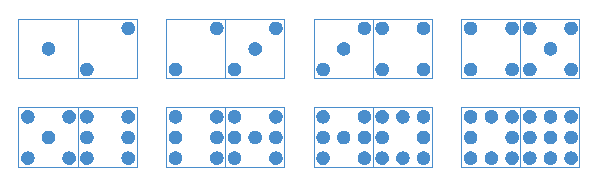
\includegraphics[width= 1\linewidth]{OC24}
		\vspace*{-10pt}
	\end{figure}
	Liệu có thể lát kín hoàn toàn một bảng vuông có kích thước $4 \times 4$ bằng những quân domino này sao cho tổng số chấm trên mỗi hàng, mỗi cột đều bằng nhau?
	\vskip 0.1cm
	\textit{Lời giải.} Có thể lát thỏa mãn điều kiện đầu bài như sau (để đơn giản ta viết số thay cho các chấm trên domino) 
	\begin{figure}[H]
%		\vspace*{-5pt}
		\centering
		\captionsetup{labelformat= empty, justification=centering}
		\begin{tikzpicture}[cackithi,scale=0.65, node font=/small]
			\draw (0,0) rectangle (4,4);
			\draw (0,2) -- (4,2) (0,3) -- (4,3) (1,0) -- (1,2) (3,0) -- (3,2) (2,4) -- (2,0);
			\draw (0.5, 0.5) node {$7$};
			\draw (0.5, 1.5) node {$8$};
			\draw (0.5, 2.5) node {$4$};
			\draw (0.5, 3.5) node {$1$};
			\draw (1.5, 0.5) node {$6$};
			\draw (1.5, 1.5) node {$7$};
			\draw (1.5, 2.5) node {$5$};
			\draw (1.5, 3.5) node {$2$};
			\draw (2.5, 0.5) node {$4$};
			\draw (2.5, 1.5) node {$3$};
			\draw (2.5, 2.5) node {$5$};
			\draw (2.5, 3.5) node {$8$};
			\draw (3.5, 0.5) node {$3$};
			\draw (3.5, 1.5) node {$2$};
			\draw (3.5, 2.5) node {$6$};
			\draw (3.5, 3.5) node {$9$};
		\end{tikzpicture}
		\vspace*{-10pt}
	\end{figure}
	Trong phần cuối của chuyên mục kỳ này, chúng tôi sẽ giới thiệu với bạn đọc ba bài toán trong kỳ thi Olympic Toán học Trẻ của Vương quốc Anh năm học $2022$. Các bài toán này phù hợp với trình độ học sinh lớp $6-8$.
	\vskip 0.1cm
	{\bf\color{cackithi} OC$\pmb{31.}$} Bốn góc trong một tứ giác có số đo là các số tự nhiên có $2$ chữ số $\overline{ab}, \overline{cd}, \overline{bd}, \overline{ac}$ như trong hình vẽ. Tìm tất cả các khả năng có thể của tập hợp bốn góc trên.
	\begin{figure}[H]
		\vspace*{-5pt}
		\centering
		\captionsetup{labelformat= empty, justification=centering}
		\begin{tikzpicture}[cackithi,scale=0.85, node font= /small]
			\draw  (5.48,-1.)-- (8.,-1.);
			\draw  (8.,-1.)-- (9.,2.);
			\draw  (9.,2.)-- (4.36,1.82);
			\draw  (4.36,1.82)-- (5.48,-1.);
			\draw [fill=white] (5.48,-1.) circle (1.5pt);
			\draw (5.8,-0.63) node {$\overline{cd}^\circ$};
			\draw [fill=white] (8.,-1.) circle (1.5pt);
			\draw (7.76,-0.57) node {$\overline{bd}^\circ$};
			\draw [fill=white] (9.,2.) circle (1.5pt);
			\draw (8.56,1.73) node {$\overline{ac}^\circ$};
			\draw [fill=white] (4.36,1.82) circle (1.5pt);
			\draw (4.95,1.57) node {$\overline{ab}^\circ$};
		\end{tikzpicture}
		\vspace*{-10pt}
	\end{figure}
	{\bf\color{cackithi}OC$\pmb{32.}$} Cho hình ngũ giác đều $ABCDE$. Vẽ hai đường tròn: một có
	tâm $A$ và bán kính $AB$, và hình kia có tâm $B$ và bán kính $BA$. Gọi $X$ là giao điểm bên trong ngũ giác của hai đường tròn.
	Hỏi số đo của $\angle DEX$ bằng bao nhiêu?
	\vskip 0.1cm
	{\bf\color{cackithi}OC$\pmb{33.}$} Seth làm $n$ viên xúc xắc giống hệt nhau bằng cách gấp $n$ bản giống như trong hình bên. Sau đó, anh ta xếp lần lượt các viên xúc xắc chồng lên nhau thành một hình tháp thẳng đứng.
	Biết rằng tổng số chấm ở mỗi một trong bốn mặt xung quanh của tháp xúc xắc đều là số lẻ. Hỏi các giá trị có thể của $n$ là bao nhiêu?
	\begin{figure}[H]
		\vspace*{-5pt}
		\centering
		\captionsetup{labelformat= empty, justification=centering}
		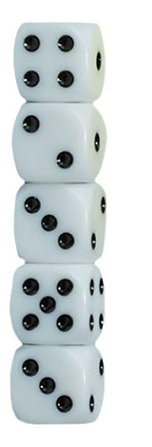
\includegraphics[height= 0.6\linewidth]{OC33}
		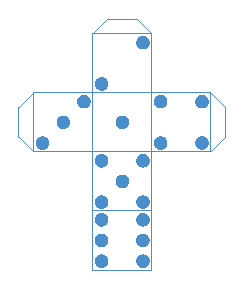
\includegraphics[height= 0.6\linewidth]{OC}
		\vspace*{-5pt}
	\end{figure}
\end{multicols}